% !TeX root = ../main.tex

\chapter{相关技术分析}

从第一章的分析可以看出,当前体系结构模拟器的研究主要是基于主流的指令集架构,依托于具体的硬件实现,从处理器功能和性能两个不同的角度对模拟器进行设计。所以本章首先分析主流指令集架构和RISC-V架构的特点,然后介绍体系结构模拟器的相关技术,最后结合本系统的设计目标--为RISC-V架构的系统软件提供移植环境并辅助进行处理器验证,提出了基于解释型的指令集模拟策略,对RISC-V架构处理器进行功能模拟。

\section{指令集架构概述}

指令集架构(Instruction Set Architecture, ISA)是计算机体系结构中定义的软硬件接口规范,是信息技术生态的原始起点\cite{刘畅2021risc}。
根据同一指令集架构,不同的厂商可以设计出性能各异的处理器,虽然生产的芯片会有成本,功耗,性能上的区别,但是它们都可以运行基于同一指令集架构开发的软件。指令集架构主要分为复杂指令集(Complex Instruction Set Computer, CSIC)和精简指令集(Reduced Instruction Set Computer,RSIC),前者使用不定长的指令设计方案,单条指令的功能实现有相当大的空间,但是由于保留了许多复杂指令,使得CPU设计变得异常繁杂,大大增加了硬件设计的时间成本和面积开销\cite{王雅婕2020用于能量计量的};而后者采用定长的指令设计方案,只保留处理器常用指令,因此指令结构较为精简,相应的硬件设计也会比较简洁。这两种指令集架构的代表分别是X86架构和ARM架构。其中X86架构因为其向下兼容的特点在PC领域占有巨大的市场份额,而ARM架构因为低功耗的特点被广泛用于嵌入式领域。这两种指令集架构的共同特点是闭源,并且授权费高昂。

% X86架构是Intel公司推出的一款复杂指令集架构,最初用于16位微处理器i8086,后来在与ARM公司的竞争中,逐步发展成为包含64位指令集的X86家族,具备向下兼容的特点,Inter公司陆续研制更加新型的处理器如i80386,Pentium4等,为了保证新处理器能够继续运行以往开发的各类应用程序以保护和继承丰富的软件资源,Intel公司所生产的所有CPU仍然继续使用X86指令集,所以它的CPU仍属于X86系列。另外除Intel公司之外,AMD和Cyrix等厂家也相继生产出能使用X86指令集的CPU,由于这些CPU能运行所有的为Intel CPU所开发的各种软件,所以电脑业内人士就将这些CPU列为Intel的CPU兼容产品。由于Intel X86系列及其兼容CPU都使用X86指令集,所以就形成了今天庞大的X86系列及兼容CPU阵容。
% % x86是由英特尔公司推出的一种复杂指令集架构,采用可变指令长度的设计。在x86诞生初期,CSIC还是业界主流,虽然在之后RSIC已经取代CSIC成为主流,但是由于英特尔公司的巨大成功以及为了软件兼容性做出的妥协,x86架构被一直保留了下来。为了克服CSIC的部分缺点,英特尔也做出了很多优化。
% % 例如,Intel 采用“微码化”先把复杂的 CISC 指令用硬件解码器翻译,变成简单的指令序列,然后再运行,采用流水线的方法,使得即使是 CISC 架构的 x86 也可以借鉴 RISC 架构的优点。但是这样也带来了额外的硬件开销,影响其性能,这是作为 CISC 架构的 x86 不得不付出的代价。


% ARM(Advanced RISC Machines)公司的主要业务是向其他 CPU 设计制造商提供知识产权(IP),并通过收取专利许可费来获取利润。ARM架构是一个精简指令集处理器架构族,由于其能耗方面的巨大优势,被广泛地用于嵌入式系统设计。在如今讲究效能比的时代,能耗成为了高端处理器市场最重要的指标,在移动通信领域,采用ARM架构的处理器具有高性能,低功耗的特点,这也使得ARM公司成为了移动通信和IOT市场的绝对霸主。
% % 支持 Thumb(16 位)/ARM(32 位)双指令集,能很好地兼容 8 位/16 位器件(Thumb 是 ARM 体系结构中一种 16 位的指令集)。指令执行采用 3 级流水线/5 级流水线技术。寻址方式灵活简单,执行效率高。指令长度固定(在 ARM 状态下是 32 位,在Thumb 状态下是 16 位)。如今,ARM 处理器占领了 32 位嵌入式处理器的大部分市场,并且是世界上使用最广泛的 32 位处理器体系结构。来自世界各地的数十家著名的半导体公司都在使用 ARM 的授权。然后通过自己的外围电路设计,开发的 ARM 处理器可用于许多领域。


% 上述两种指令集架构分别是CISC和SISC的代表,他们共同的特点是,闭源且授权费高昂,当其他拿到授权的公司生产的芯片使得Intel和ARM公司受到威胁时,Intel和ARM完全可以拿起专利的大棒停止授权。


\section{RISC-V架构}

第五代精简指令集(RISC-V, Reduced Instruction Set Computer - Five)于2011年诞生于加州大学伯克利分校\cite{余振波2020基于},由David.Paterson教授团队设计,由于其开放性和包容性,以及充分发挥的后发优势,如今的RISC-V已经成为行业实施的的标准开源指令集架构。RISC-V的指令集使用模块化的方式进行组织,包含标准拓展的RISC-V指令集组成如表~\ref{tab:isa-general}所示。
\begin{table}[H]
  \centering
  \caption{RISC-V指令集模块}
  \label{tab:isa-general}
  \renewcommand\arraystretch{1.2}
  \begin{tabular}{cccl}
    \toprule
指令集类型 & 类型简写	& 指令数 &	说明 \\
    \midrule
    \multirow{4}{*}
    {基本指令集} &	
      RV32I &	47	& \multicolumn{1}{m{8.5cm}}{基本整数指令集,包含算数指令、访存指令、环境调用等指令} \\ \cline{2-4}
      & RV32E	& 47	& \multicolumn{1}{m{8.5cm}}{RV32I指令集简化版本,专为嵌入式设计} \\ \cline{2-4}
      & RV64I	& 59	& \multicolumn{1}{m{8.5cm}}{整数指令} \\ \cline{2-4}
      & RV128I	& 71	& \multicolumn{1}{m{8.5cm}}{整数指令} \\ \hline
    \multirow{6}{*}
    {扩展指令集} &
      M	& 8	& \multicolumn{1}{m{8.5cm}}{乘除扩展} \\ \cline{2-4}
      & A	& 11	& \multicolumn{1}{m{8.5cm}}{原子扩展}\\ \cline{2-4}
      & F	& 26	& \multicolumn{1}{m{8.5cm}}{单精度浮点扩展}\\ \cline{2-4}
      & D	& 26	& \multicolumn{1}{m{8.5cm}}{双精度浮点扩展}\\ \cline{2-4}
      & C	& 46	& \multicolumn{1}{m{8.5cm}}{压缩指令扩展}    \\
    \bottomrule
  \end{tabular}
\end{table}


其中, RV32 和 RV64 表示寄存器的位宽,决定了处理器寻址范围的大小。基本整数指令集是所有RISC-V架构设计方案都必须实现的最小子集,其余的统称为拓展指令集,是可选的。
% 在该指令集架构中基本整数指令集(Integer)使用简写“I”来表示 ,该模块包含了整数计算指令、整数加载指令、整数存储指令和控制流指令,实现基本整数指令集是任何一款基于 RISC-V 指令集架构的微处理器所必须满足的;标准的整数乘法和除法扩展(Multiply)使用简写“M”表示,指令功能是对整数寄存器中保存的值进行乘法和除法操作;标准的原子指令扩展(Atomic)使用简写“A”表示,添加原子性的读取、修改和写入内存的指令,保证了多核处理器间的访存一致性;单精度浮点扩展(Float)使用简写“F”来表示,该扩展增加了浮点寄存器、单精度计算指令和单精度加载以及存储指令;标准的双精度扩展(Double)使用简写“D”表示,扩展了浮点寄存器,并且增加了双精度计算、加载和存储指令。整数基数集加上四个标准扩展(即“IMAFD”)可以缩写为“G”,表示实现通用标量指令集。为了提高代码密度,RISC-V架构也提供可选的“压缩”指令子集(Compress),由英文字母“C”表示。压缩指令的指令编码长度为16比特,而普通的非压缩指令的长度为32比特。


RISC-V 指令集架构所使用的定点通用寄存器如表\ref{tab:xpr}所示,浮点通用寄存器如表\ref{tab:fpr}所示。
\begin{table}[H]
  \centering
  \caption{RISC-V定点通用寄存器}
  \label{tab:xpr}
  \begin{tabular}{cccc}
    \toprule
寄存器 &	助记符	& 描述 &	调用与被调用\\
    \midrule
    x0 & zero & 硬编码为 0 & -\\
    x1 & ra & 返回地址寄存器 & 调用者\\
    x2 & sp & 堆栈指针寄存器 & 被调用者\\
    x3 & gp & 全局指针寄存器 & -\\
    x4 & tp & 线程指针寄存器 & -\\
    x5 & t0 & 临时/备用链接寄存器 & 调用者\\
    x6-7 & t1-2 & 临时寄存器 & 调用者\\
    x8 & s0/fp & 保存的寄存器/帧指针 & 被调用者\\
    x9 & s1 & 保存的寄存器 & 被调用者\\
    x10-11 & a0-1 & 函数参数/返回值寄存器 & 调用者\\
    x12-17 & a2-7 & 函数参数寄存器 & 调用者\\
    x18-27 & s2-11 & 保存的寄存器 & 被调用者\\
    x28-31	& t3-6 & 临时寄存器 & 调用者\\
    \bottomrule
  \end{tabular}
\end{table}


\begin{table}[h]
  \centering
  \caption{RISC-V浮点通用寄存器}
  \label{tab:fpr}
  \begin{tabular}{cccc}
    \toprule
寄存器 &	助记符	& 描述 &	调用与被调用\\
    \midrule
    f0-7 & ft0-7 & 浮点临时寄存器 & 调用者\\
    f8-9 & fs0-1 & 浮点保存寄存器 & 被调用者\\
    f10-11 & fa0-1 & 浮点参数/返回值寄存器 & 调用者\\
    f12-17 & fa2-7 & 浮点参数寄存器 & 调用者\\
    f18-27 & fs2-11 & 浮点保存寄存器 & 被调用者\\
    f28-31 & ft8-11 & 浮点临时寄存器 & 调用者\\
    \bottomrule
  \end{tabular}
\end{table}


RISC-V指令集有以下特点:


(1) 完全开源,使用RISC-V架构无需获取授权;


(2) 模块化的指令集设计,针对不同的应用场景,可以选择支持不同组合的指令集模块,有很好的灵活性。


(3) 提供可配置的通用寄存器组。


(4) 提供规整的指令编码格式,在指令格式中寄存器索引位置对齐,方便译码器硬件实现。


(5) 极简的设计哲学,摒弃了分支延迟槽,条件码执行等特性,极大地简化了硬件电路的布局。


(6) 方便用户自定义,用户可以对中断系统进行定制,并且还可以实现自定义的拓展指令。


% (2) 适用于直接本机硬件实现,而不仅仅是模拟或二进制转换的真正的 ISA;


% (3) 避免在微体系结构(例如:顺序、乱序、解耦微处理器)或微技术(例如:全定制、ASIC、FPGA)实现中“过渡架构”,并且在这些实现中更有效率的一款指令集架构;


% (4) RISC-V 可以将指令集架构分成一个小的基本整数指令集架构,具备可选的标准扩展,以支持通用软件开发,并且可用于自定义加速器开发或教学;


% (5) 支持 2008 年修订的浮点 IEEE-754 标准;


% (6) 一款支持广泛的用户级 ISA 扩展和专用变体的指令集架构;


% (7) 适用于应用程序,操作系统内核以及计算机硬件实现 32 位或 64 位地址空间变体;


% (8) 该指令集架构支持包括异构多核处理器在内高度并行多核的实现;


% (9) 可供用户选则的可变长度指令格式,对可用指令编码空间进行扩展,指令集架构所支持的可选密集指令编码用以提高性能,减小静态代码大小以及提升能量效率;


% (10)完全可虚拟化的 ISA,可简化虚拟机管理程序开发;


% (11)一个简化了新的管理员级和管理程序级的 ISA 设计。

RISC-V架构为软件开发人员提供了开源的指令集规范,也为硬件设计人员提供的便利的指令集模块支持,厂家可以根据自身产品特性选择适合自己的组合模块。这样的指令级架构演化模式充分调动了软硬件开发者的热情,也吸引了众多商业芯片厂商的目光,同时极大地降低了处理器的设计门槛,能够方便研究者进行零成本的创新实践。按照如今RISC-V开源社区的发展态势,有望在新兴的 AI 与 IoT 领域中对ARM 的统治地位形成挑战\cite{邓紫珊2020基于},这同时也是我国能在芯片设计领域打破技术壁垒的良好契机。
% 同时也为中国在芯片设计领域打破国外技术垄断提供了契机。
\section{体系结构模拟器}
模拟器是体系结构量化分析的重要手段,对架构设计、芯片开发有重要的指导作用。基于模拟器辅助进行集成电路设计可以追溯到1980年代\cite{mukherjee2002performance},自此模拟器便一直是处理器设计过程中不可或缺的工具。在芯片开发项目中,体系结构模拟器的具体作用如图~\ref{fig:sim-func}所示:
\begin{figure}[h]
  \centering
  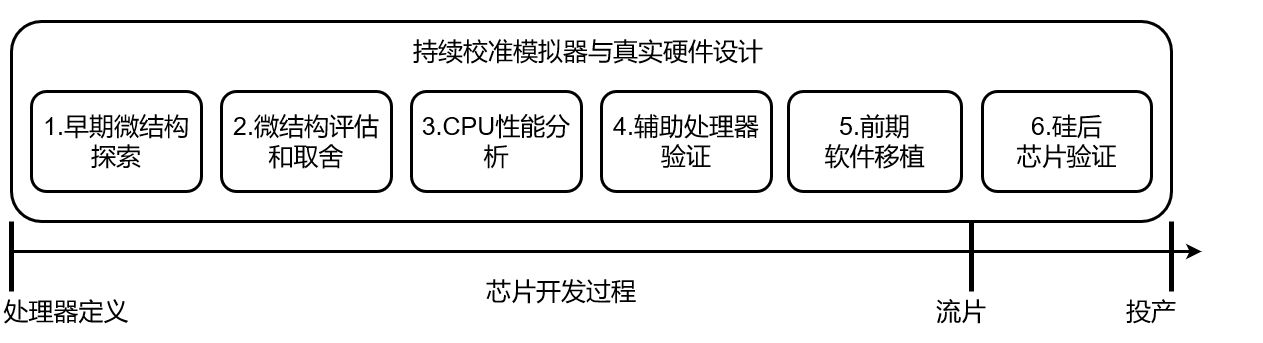
\includegraphics[width=1.0\textwidth]{sim_func.png}
  \caption{体系结构模拟器在CPU开发流程中的作用}
  \label{fig:sim-func}
\end{figure}


1) 在芯片开发早期,基于体系结构模拟器可以进行微结构探索和粗粒度微结构定义,此时模拟器的开发抽象层次较高。


2) 随着处理器设计的不断推进和模拟器的不断完善,基于模拟器可以持续对芯片微结构进行评估、修改和取舍。


3) 当模拟器趋于成熟,可以对微结构、多核互联系统、一致性协议等进行详细性能分析,基于分析结果对微结构进行微调。


4) 在对处理器逻辑设计进行验证的阶段,模拟器可以作为参考模型辅助进行验证,可以快速定位逻辑设计错误。


5) 在未流片之前基于模拟器就可以开展系统软件开发和适配工作,在芯片流片结束后以最快速度启动系统软件。


6) 流片结束后,基于模拟器可以辅助进行芯片硅后验证环境的搭建以及测试用例编写工作\cite{brooks2000wattch}。为了保证模拟器可以顺利辅助进行处理器设计,在整个芯片开发过程中,需要持续对模拟器进行校准,通过持续对比模拟器和寄存器传输层(Register-Transfer Level, RTL)之间的差别,可以互相校准并发现模拟器或者RTL的设计错误\cite{hourui}。


\begin{figure}[h]
  \centering
  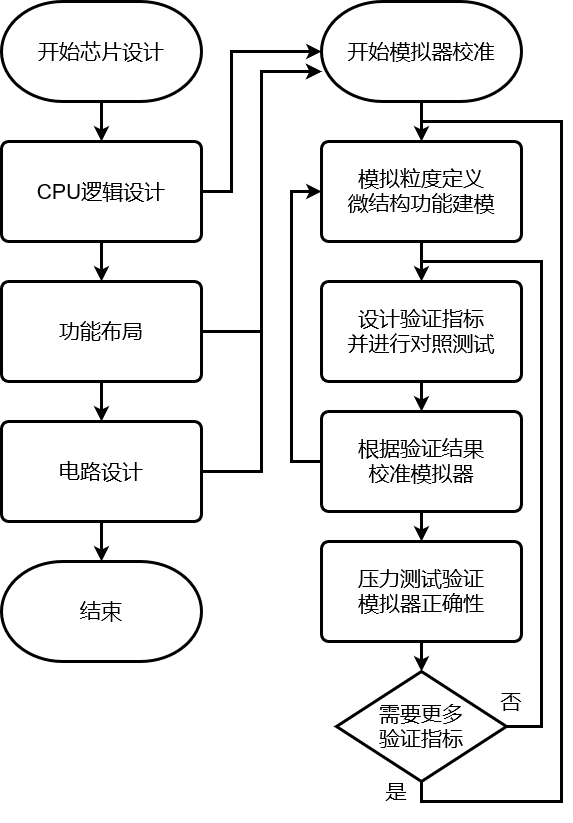
\includegraphics[width=0.5\textwidth]{sim_develop.png}
  \caption{体系结构模拟器开发流程图}
  \label{fig:sim-dev-process}
\end{figure}

使用体系结构模拟器进行辅助开发的基本流程如图~\ref{fig:sim-dev-process}所示。首先,需要对模拟的粗细粒度进行定义,是功能模拟还是性能模拟,然后需要对实际的硬件设计进行建模,将无需模拟的部分进行抽象,使用软件手段封装成黑箱,这部分不必过分关心硬件的实现细节,只需对输入输出作明确的定义。为了达到所需的模拟精度,需要对模拟器和真实硬件进行行为比对,此外,建模过程中所选的具体算法需要达到对模拟器的性能要求。确定好的模拟方案,完成建模,选定合适的实现算法后,进行程序设计。等确定了程序的正确性后,就可以使用该模拟器进行后续的工作,如对处理器系统软件的预开发移植,或者是对模型本身进行评价或研究,也可以是对模拟的目标系统性能作出评价。


根据模拟粒度可以将体系结构模拟器分为两类,功能模拟器(指令集模拟器Instruction  Set  Simulator, ISS)和性能模拟器(时钟周期精确模拟器)\cite{单磊2012大规模并行片上系统的分布式并行模拟关键技术研究}。ISS只模拟目标系统的指令集体系结构,比如寄存器状态、指令语义、存储器状态等功能特性;性能模拟器除了模拟功能特性外,还模拟目标系统的微体系结构,比如流水线、分支预测等\cite{cachecengcideng}。

对于指令集模拟器ISS,在设计过程中,需要充分考虑指令集模拟策略以及模拟器驱动方式。指令集模拟策略是ISS设计的基础,它决定了模拟器的性能,同时也会影响模拟器调试模块的功能实现。指令集模拟策略分为两种:基于解释型和基于编译型。下面将详细介绍这两种模拟策略。
% 首先通过对实际硬件系统建模来将之具体化。建模与具体化的过程中必须保证所建模型的结构与实际硬件系统相近或一致,以确保所建模型的精确性,只有精确度较高的模型才能真实的模拟出硬件系统的行为,最终获得正确的结果。在对硬件系统的建模过程中,需要考虑所选择的算法是否合适。评价一种算法是否合适的准则在于是否符合模拟的要求和硬件系统的特征。为了保证最终的模拟精度,必须确保所选择算法的精度够高,稳定性够好。选定合适的算法后,进行程序设计,即用程序语言将模型描述出来。待确定程序模型的正确以后,就可以用这个模型来进行模拟实验,得到相应的结果。最后分析模拟结果,结果分析既可以是针对模型本身的数据,



\subsection{解释型指令集模拟}
解释型指令集模拟器的最大的特点在于直接将硬件行为映射到软件,从而模拟出真实的硬件环境,由于其对指令进行逐条翻译,使得指令流程控制很容易实现\cite{jump,蔡启先2010mips64}。ISS的指令控制流程通常是取指-译码-执行的循环,如图~\ref{fig:ISS-interprete}所示。
\begin{figure}[h]
  \centering
  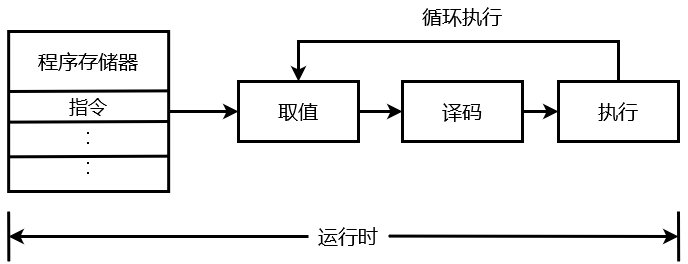
\includegraphics[width=0.7\textwidth]{ISS-interprete.png}
  \caption{解释型ISS工作流程}
  \label{fig:ISS-interprete}
\end{figure}


1) 取指:模拟器取出目标程序的单条指令;


2) 译码:模拟器对目标指令进行翻译,得到指令对应的功能函数; 


3) 执行:模拟器执行目标指令所对应的功能函数,完成功能函数中定义的软硬件行为。


解释型指令集模拟器的工作流程使得模拟器设计比较简单,易于建模和实现,且灵活性较好,模拟精度高。但是由于模拟器通过软件行为对指令进行逐条译码,相较于真实硬件电路效率太低\cite{gutierrez2014sources},所以解释型ISS的模拟速度一般不是很高。


\subsection{编译型指令集模拟}
基于编译型的ISS通过对译码过程的改进,大幅度提升了模拟的效率,编译型ISS采用二进制翻译技术\cite{李剑慧2007动态二进制翻译与优化技术研究}将目标指令翻译成宿主机可识别的指令来完成对目标机状态的模拟。根据译码过程处于编译还是运行时,又可分为静态编译型指令集模拟器(Static Compiled ISS)和动态编译型指令集模拟器(Dynamic Compiled ISS)\cite{刘晓燕2014一种}。由Zhu and Gajski\cite{zhu1999retargetable}给出的静态编译型指令集模拟器将本处于运行时的指令译码过程转移至编译时,如图~\ref{fig:static-ISS}所示。首先使用交叉编译器将目标程序编译成目标机架构的二进制文件,接着使用代码生成器进行优化,最终翻译为宿主机二进制文件,由宿主机直接运行。这种基于二进制翻译的指令集模拟策略拥有很高的执行效率,运行速度接近宿主机。
\begin{figure}[h]
  \centering
  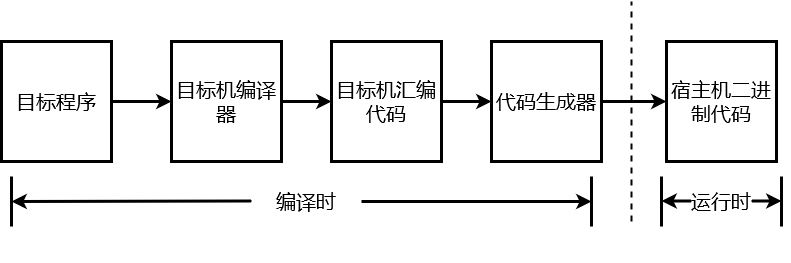
\includegraphics[width=0.9\textwidth]{static-ISS.png}
  \caption{静态编译型ISS工作流程}
  \label{fig:static-ISS}
\end{figure}


动态编译型ISS的典型代表为Embra\cite{witchel1996embra}及Shade\cite{cmelik1995shade},其工作流程如图~\ref{fig:dynamic-ISS}所示:
\begin{figure}[h]
  \centering
  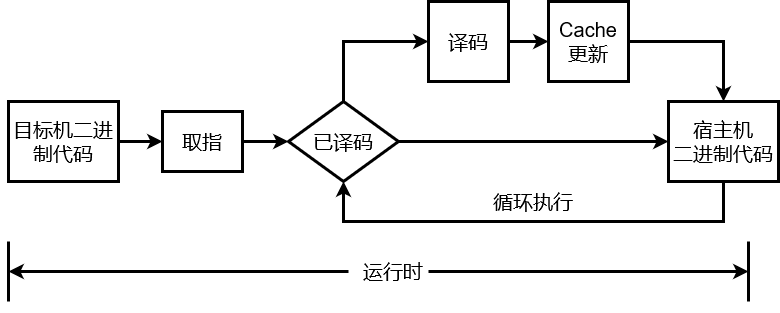
\includegraphics[width=0.9\textwidth]{dynamic-ISS.png}
  \caption{动态编译型ISS工作流程}
  \label{fig:dynamic-ISS}
\end{figure}


% 其借鉴了iCache的思想,模拟器取指之后判断该条指令是否是第一次执行,若是,那么对其进行译码,并将译码信息保存到Cache中,然后执行;若不是,则直接在 Cache 中调用该指令的译码信息执行。由于该技术在程序运行时进行指令译码,因此很难进行代码优化。

\subsection{模拟器技术选型}
% 模拟器开发投入很大,要持续与RTL进行校准\cite{gao2007simos}。模拟器的开发首先是一项软件工程,因此好的软件架构是模拟器成功的首要条件,相比而言计算机体系结构的知识也非常重要但是次要的\cite{desikan2001sim}。AMD模拟器的微结构代码约有10万行,其他结构包含共享库约有40万行代码,因此模块化的设计、良好的代码接口、使用源代码管理工具等必不可少。在资源不足的情况下,基于开源模拟器开发模拟器也是不错的选择。
% 模拟器校准时,需要通过微程序进行充分验证\cite{gao2007simos},此时可以跟验证团队紧密合作,共享验证微程序。性能模拟器编写语言一般选择兼顾开发和执行效率的C++,其次是C语言。为了加速模拟器仿真速度,模拟部件尽量并行执行,且要尽可能支持可移植性。
本模拟器的开发目标是对RISC-V架构处理器进行功能模拟,模拟的粒度是单条RISC-V汇编指令,属于指令集功能模拟器,用于系统软件的移植开发和测试工作。为了兼顾开发和执行效率,本模拟器采用面向对象的设计方法,使用C++实现前后端代码框架,采用解释型的指令集模拟策略,最终完成了RISC-V指令集功能模拟器的开发。


\section{本章小结}
本章节主要介绍了RISC-V指令集架构的特点以及体系结构模拟器的相关技术。对体系结构模拟器的功能和开发流程做了介绍,并对几种常见的模拟器类型作了分析对比,其中详细介绍了指令集模拟器ISS,对指令集模拟器的模拟流程以及两种指令集模拟策略的优缺点进行了分析,最终结合实际芯片开发项目需求,以及RISC-V指令集架构的特点,拟定了本次模拟器的设计方案:采用基于解释性的指令集模拟策略,方便进行调试功能的实现,并且结合了动态编译型ISS的译码优化策略,提高模拟器执行效率。